\section{Introduction}

In this chapter we focus on the concept of local features and its usage within a 3d reconstruction pipeline. Precisely, as we introduced in the previous chapter we empathize on the classical features matching pipeline, or Wide Baseline Stereo (WBS) algorithm which can be decomposed in several sub-tasks to be processed independently. First, in section~\ref{sec:local_detectors} we analyze the problem of the detection of points of interest in the scene, then, in section~\ref{sec:local_descriptors} how to describe the points in order to match them between different views robustly.

Local features is one of the most studied topics by the Computer Vision community which resulted to a wide list of different applications such as image stitching, camera calibration and obviously for scene reconstruction, which is the topic of this thesis. Local features detection can be formally described as the problem of finding discriminative regions in an image from which several properties as the location, orientation or the shape. On the other hand, the task to extract local features descriptors consist in computing embeddings from the small image patches which later are used for the matching task as seen in the WBS pipeline figure~\ref{fig:wbs-pipeline}. Thus, the scope of this thesis is just to cover and propose novel solutions for the two initial steps of the classic pipeline within the scene reconstruction context.

Traditionally, several of the proposed methods to solve features detection use low level image processing techniques that brought to a wide number of well founded algorithms based on robust and handcrafted methods~\cite{SIFT, ORB}, as can be seen in figure~\ref{fig:feature_detection_example}. However, in this thesis we propose a novel approach for keypoints detection task that combines handcrafted and learned CNN filters within a shallow multi-scale architecture. Handcrafted filters provide anchor structures for learned filters, which localize, score and rank repeatable features. Scale-space representation is used within the network to extract keypoints at different levels. We design a loss function to detect robust features that exist across a range of scales and to maximize the repeatability score. The proposed method, named Key.Net model is trained on data synthetically created from ImageNet~\cite{AlexNet2012} and evaluated on HPatches benchmark~\cite{HPatches}. Results are provided to show that the approach outperforms state-of-the-art detectors in terms of repeatability, matching performance and complexity.

Additionally, it has recently been demonstrated that local feature descriptors based on convolutional neural networks (CNN) can significantly improve the matching performance and with it the final 3d reconstruction of a scene. Previous work on learning such descriptors has focused on exploiting pairs of positive and negative patches to learn discriminative CNN representations. In this thesis, we propose a new method that utilizes triplets of training samples, together with in-triplet mining of hard negatives. We show that the method achieves state of the art results, without the computational overhead typically associated with mining of negatives and with lower complexity of the network architecture. The approach is compared to recently introduced convolutional local feature descriptors, and demonstrate the advantages of the proposed methods in terms of performance and speed.

\begin{figure}
    \centering
    \subfloat[\centering]{{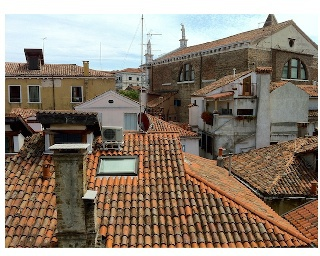
\includegraphics[width=5cm]{main/chapter02/figures/sift_basic_0.jpg} }}
    \qquad
    \subfloat[\centering]{{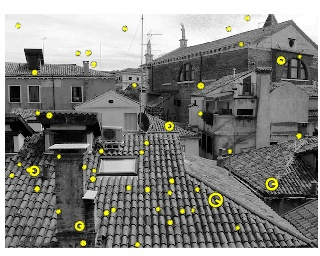
\includegraphics[width=5cm]{main/chapter02/figures/sift_basic_2.jpg} }}
    \caption[Local feature detection using VLFeat]{\textbf{Local feature detection using VLFeat.} Example showing the result of a local features detection algorithm using the VLFeat library~\cite{vedaldi08vlfeat} with the SIFT~\cite{SIFT} detector. \textbf{Left:} the original RGB image. \textbf{Right:} the image in grayscale containing the found keypoints represented as circles, where the radius show the estimated size of the keypoint. Image is courtesy of the VLFeat examples website.}
    \label{fig:feature_detection_example}
\end{figure}

\section{Feature Detection}
\label{sec:local_detectors}

Recent advances in local feature detectors and descriptors has led to remarkable improvements in areas such as image matching, object recognition, self-guided navigation or 3D reconstruction. Although the general direction of image matching methods is moving towards learned based systems, the advantage of learning methods over handcrafted ones has not been clearly demonstrated in keypoint detection \cite{Karel_Vedaldi_BMVC_18} bringing initial approximations less efficient and with a high computational cost.
%In particular, Convolutional Neural Networks (CNNs) were able to significantly reduce matching error in local descriptors~\cite{HPatches}, despite the impractical inefficiency of the initial techniques~\cite{MatchNet15,Zagoruyko15}. These works stimulated further research efforts and resulted in improved efficiency of CNN based descriptors, on the contrary, on top of the limited success of learned detectors, a general trend towards dense rather than sparse representation and matching put aside local feature detectors. 
However, the growing popularity of augmented reality (AR) headsets, as well as AR smartphone apps, has drawn more attention to reliable and efficient local feature detectors that could be used for surface estimation, sparse 3D reconstruction, 3D model acquisition or objects alignment, among others. \par

Traditionally, local feature detectors were based on engineered filters. For instance, approaches such as Difference of Gaussians~\cite{SIFT}, Harris-Laplace or Hessian-Affine~\cite{mikolajczykIJCV2004} use combinations of image derivatives to compute feature maps, which is remarkably similar to the operations in trained CNN's layers. Intuitively, with just a few layers, a network could mimic the behavior of traditional detectors by learning the appropriate values in its convolutional filters. However, the improvements upon handcrafted detectors offered by recently proposed fully CNN based methods~\cite{LIFT,DeTone_MagicPoint17,Karel_Vedaldi_ECCV_16, Zhang_Felix_CVPR_17,OnoSerra18} are limited in terms of widely accepted metrics such as repeatability which measures the closeness between the detected keypoint location and its ground truth. In contrast to the method that we propose later, in addition to the keypoint location, in some cases the estimation of the scale (or surrounding region) and even the affine transformation is required. However, those methods usually lack in terms of accuracy when estimating the affine parameters of the feature regions. Robustness to scale variations seems particularly problematic while other parameters such as dominant orientation can be regressed well by CNNs~\cite{Yi_Verdie_Fua_Lepetit_CVPR16, LIFT}.

These problems in previous approaches motivates our novel architecture, termed Key.Net, that makes use of handcrafted and learned filters as well as a multi-scale representation to identify keypoints at different scales. 
The Key.Net architecture is illustrated in figure~\ref{keynet_fig:net_architecture}. Introducing handcrafted filters, which act as soft anchors, makes possible to generate a model with fewer parameters that state of the art detectors while maintaining the performance in terms of repeatability. The model operates on a multi-scale representation of full-size images and returns a response map containing a keypoint score for every pixel. The multi-scale input allows the network to propose stable keypoints across scales thus providing robustness to scale changes considering that the network does not explicitly predict the affine parameters for the scale. 

Ideally, a robust detector is able to propose the same keypoints for images that undergo different geometric or photometric transformations. A number of related works have focused their objective function to address this issue, although they were based either on local patches~\cite{Karel_Vedaldi_ECCV_16, Zhang_Felix_CVPR_17} or global map regression loss~\cite{detone2017superpoint, TILDE, OnoSerra18}. In contrast, we extend the covariant constraint loss used in previous works to a new objective function that combines local and global information in order to predict more stable keypoints across the different scales. The Key.Net architecture produces as an output a response map which needs an operator to extract discrete keypoint locations to evaluate the geometric loss function. For this reason, we design a fully differentiable operator, Multi-scale Index Proposal, that proposes keypoints at multi-scale regions. We extensively evaluate the method in recently introduced HPatches benchmark~\cite{HPatches} in terms of accuracy and repeatability according to the protocol from~\cite{mikolajczykpami2005}.\\

\noindent In summary, the contribution presented in this section is a multi-scale feature detection method with a shallow architecture based on:

\setlist{nolistsep}
\begin{enumerate}
    \item the Key.Net network that generates a response map for those potential regions in the input image that might contain a keypoint.
    \item a differentiable operator to extract and rank the stable keypoints across the scales.
\end{enumerate}

\noindent The rest of the section is organized as follows. A revision in keypoint detection is shown in section~\ref{keynet_sec:related_work}. Section~\ref{keynet_sec:architecture} presents the proposed hybrid Key.Net architecture of handcrafted and learned CNNs filters and section~\ref{keynet_sec:loss_functions} introduces the loss. Implementation and experimental details are given in section~\ref{keynet_sec:experimental_evaluation} and the results are presented in section~\ref{keynet_sec:results}.


%----------------------------------------------------------------------------------------
%	Section: Related Work
%----------------------------------------------------------------------------------------
\subsection{Related Work in Feature Detection}
\label{keynet_sec:related_work}

There are many surveys that extensively discuss feature detection methods~\cite{Karel_Vedaldi_BMVC_18, TuytelaarsMikolajczyk2007}. 
In this section related works are presented and organized in two main categories: handcrafted and learned based detectors. 

%----------------------------------------------------------------------------------------
%	Subsection: Handcrafted Detectors
%----------------------------------------------------------------------------------------

\subsubsection{Handcrafted Detectors}
Traditional feature detectors localize geometric structures through engineered algorithms, which are often referred to as handcrafted. Harris \cite{Harris} and Hessian \cite{Hessian} detectors used first and second order image derivatives to find corners or blobs in images. Those detectors were further extended to handle multi-scale and affine transformations \cite{mikolajczykIJCV2004, comparasionofdetector}. Region based methods such as SIFT \cite{SIFT} looked for blobs over multiple scale levels, and MSER \cite{MSER} segmented and selected stable regions as keypoints. Later, SURF \cite{SURF} accelerated the detection process by using integral images and an approximation of the Hessian matrix; and ORB~\cite{ORB} proposed an alternative to SIFT by proposing an oriented version the FAST~\cite{FAST} detector. Multi-scale improvements were proposed in KAZE \cite{KAZE} and its extension, A-KAZE \cite{AKAZE}, where Hessian detector was applied to a non-linear diffusion scale space in contrast to widely used Gaussian pyramid. Although corner detectors proved to be robust and efficient, other methods seek alternative structures within images.

%----------------------------------------------------------------------------------------
%	Subsection: Learned Detectors
%----------------------------------------------------------------------------------------

\subsubsection{Learned Detectors}
The success of learned methods in general object detection and feature descriptors motivated the research community to explore similar techniques for feature detectors. 
FAST \cite{FAST} was one of the first attempts to use machine learning to derive a corner keypoint detector. Further works extended FAST by optimizing it \cite{FASTER}, adding a descriptor \cite{BRISK} or orientation estimation \cite{ORB}.

Latest advances in CNNs also made an impact on feature detection. TILDE~\cite{TILDE} trained multiple piece-wise linear regression models to identify interest points that are robust under severe weather and illumination changes. DNet~\cite{Karel_Vedaldi_ECCV_16} introduced a new formulation to train a CNN based on feature covariant constraints. 
Previous detector was extended in~\cite{Zhang_Felix_CVPR_17} (TCDET) by adding predefined detector anchors, showing improved stability in training. In~\cite{DeTone_MagicPoint17} were presented two networks, MagicPoint, and MagicWarp, which first extracted salient points and then a parameterized transformation between pairs of images. MagicPoint was extended in \cite{detone2017superpoint} to SuperPoint, which included a salient detector and descriptor.
LIFT \cite{LIFT} implemented an end-to-end feature detection and description pipeline, including the orientation estimation for every feature. Quadruple image patches and a ranking scheme of point responses as cost function were used in \cite{savinov2016quad} to train a neural network. In \cite{Georgakis_Karanam_CVPR18}, authors proposed a pipeline to automatically sample positive and negative pairs of patches from a region proposal network to optimize jointly point detections and their representations. Recently, LF-Net \cite{OnoSerra18} estimated position, scale and orientation of features by optimizing jointly the detector and descriptor.

% In addition to the above presented learned detectors, CNN architectures also were deployed to optimize the matching stage. \cite{Hartmann_Havlena_CVPR14} learned to predict which features and descriptors were matchable. More recently, \cite{Yi_Trulls_Good_Corr_CVPR18} introduced a network to learn to find good correspondences for wide-baseline stereo. Furthermore, other CNNs also studied to perform tasks beyond detection or matching. In \cite{Yi_Verdie_Fua_Lepetit_CVPR16}, the architecture assigned orientations to interest points and AffNet \cite{Mishkin_Radenovic_Matas_AffNet_18} used the descriptor loss to learn to predict the affine parameters of a local feature.


%----------------------------------------------------------------------------------------
%	Subsection: Key.Net Architecture
%----------------------------------------------------------------------------------------

\newpage
\subsection{Key.Net Architecture}
\label{keynet_sec:architecture}

In this section we present a method to detect keypoints which attempts to combine the strong points of both handcrafted and learned-based approaches with the aim to obtain results comparable to the best learned-based detectors with the efficiency and low cost of hand-crafted solutions. The proposed architecture, named Key.Ney, can be seen in figure~\ref{keynet_fig:net_architecture}.

%----------------------------------------------------------------------------------------
%	Subsubsection: Handcrafted Filters
%----------------------------------------------------------------------------------------

\begin{figure}
\centering
\hspace*{-1cm}    
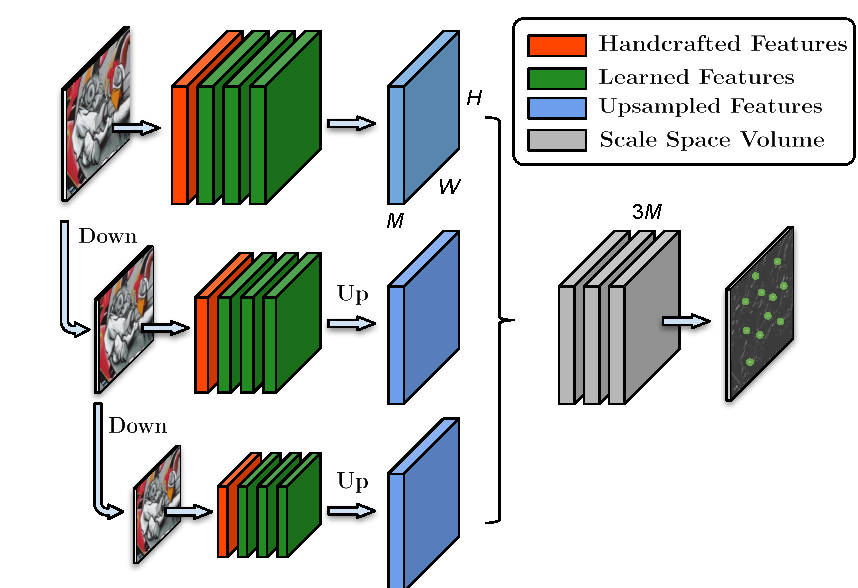
\includegraphics[width=\linewidth]{main/chapter02/figures/keynet_inference.pdf}
\vspace{-0.20cm}
\caption[Features detection architecture]{\textbf{Features detection architecture.} The proposed Key.Net architecture combines handcrafted and learned filters to extract features at different scale levels. Feature maps are upsampled and concatenated. Last learned filter combines the Scale Space Volume to obtain the final response map.}
\label{keynet_fig:net_architecture}
\end{figure}

\subsubsection{Handcrafted and Learned Filters}
\label{sec:handcrafted_filters}
The design of the handcrafted filters is inspired by the success of Harris \cite{Harris} and Hessian \cite{Hessian} detectors, which used first and second order derivatives to compute the salient corner responses. A complete set of derivatives is called {\em LocalJet}~\cite{Koendering-FlorackLocalJet} and they approximate the signal in the local neighborhood as known from Taylor expansion:
\begin{equation}
I_{i_1,\ldots,i_n}=I_0\ast\partial_{i_1,\ldots,i_n}g_{\sigma}(\vec{x}),
\label{eq:Taylor}
\end{equation}
where $g_{\sigma}$ denotes a Gaussian of width $\sigma$ centered at $\vec{x}=\vec{0}$, and $i_n$ denotes the derivative direction and order. Since higher order derivatives i.e., $n>2$ are sensitive to noise and require large kernels, the subset of \textit{LocalJet} that we have considered, includes derivatives and their combinations up to the second order only: 

\begin{itemize}
	\item \textbf{First Order}. From image $I$ we derive $1$st order gradients $I_x$ and $I_y$. In addition, we compute $I_x*I_y$, ${I_x}^2$ and ${I_y}^2$ as in the second moment matrix of Harris detector~\cite{Harris}.
    \item \textbf{Second Order}. From image $I$, $2$nd order derivatives $I_{xx}$, $I_{yy}$ and $I_{xy}$ are also included as in the Hessian matrix used in Hessian and DoG detectors \cite{HarrisLaplace,SIFT}.  We also add $I_{xx}*I_{yy}$ and $I_{xy}^2$ because of the performance boost that induce in Hessian detectors.
\end{itemize}

In addition we include a convolutional layer with $M$ learnable filters, a batch normalization layer and a ReLU activation function in order to complement the handcrafted features.
The hardcoded filters reduce the number of total learnable parameters to train the architecture, improving the stability and convergence during backpropagation.

\subsubsection{Multi-scale Pyramid }
\label{sec:pyramid}

The design of the proposed architecture has been done to be robust to small scale changes without the need for computing several forward passes and iterate over the scale space. As illustrated in figure~\ref{keynet_fig:net_architecture}, the network includes three scale levels of the input image which is blurred and downsampled by a factor of $1.2$. All the feature maps resulting from the handcrafted filters are concatenated to feed the stack of learned filters in each of the scale levels. All three streams share the weights, such that the same type of anchors result from different levels and form the set of candidates for final keypoints. Feature maps from all scale levels are then upsampled, concatenated and fed to the last convolutional filter to obtain the final response map. 

%----------------------------------------------------------------------------------------
%	Subsection: Loss Functions
%----------------------------------------------------------------------------------------

\subsection{Geometric Loss Function}
\label{keynet_sec:loss_functions}

In the proposed architecture, given an image it produces a response map that will be used later to extract the keypoints needed by the classical scene reconstruction pipeline. The learning process of the parameters in our architecture will be based on a geometric loss function which needs to be very carefully designed in order to backpropagate the gradients through the entire pipeline.

In supervised training, the loss function relies on the ground truth. In the case of keypoints, ground truth is not well defined as keypoint locations are useful as long as they can be accurately detected regardless of geometric or photometric image transformation. Some learned detectors~\cite{Karel_Vedaldi_ECCV_16,savinov2016quad,OnoSerra18} train the network to identify keypoints without constraining their locations, where only the homography transformation between images is used as ground truth to calculate the loss as a function of keypoints repeatability. 

Other works~\cite{TILDE,detone2017superpoint,Zhang_Felix_CVPR_17} show the benefits of using anchors to guide their training which work as a reference respect to the potential neighbours keypoints. Although anchors make the training more stable and lead to better results, they prevent the network from proposing new keypoints in case there is no anchor in the proximity. In contrast, the handcrafted filters in Key.Net provide a weak constraint with the benefit of the anchor-based methods while allowing the detector to propose new stable keypoints. The proposed approach, only takes the geometric transformation between images is required to guide the loss.


%----------------------------------------------------------------------------------------
%	Subsubsection: Multi-scale Index Proposal Layer
%----------------------------------------------------------------------------------------

\subsubsection{Index Proposal Layer}
\label{keynet_sec:single_index_proposal_layer}

This section introduces the Index Proposal (IP) layer, the differentiable operator used as base to extract the sub-pixel coordinates of the keypoints from the produced response maps by the network. The operator is later extended to its multi-scale version in section \ref{keynet_sec:multi_index_proposal_layer} to enforce the detection across the different scale in the features domain. 

Extracting coordinates for training keypoint detectors has been widely studied and showed great improvements: \cite{LIFT, Karel_Vedaldi_ECCV_16, Zhang_Felix_CVPR_17} extracted coordinates in reference to the patch size, SuperPoint \cite{detone2017superpoint} used a channel-wise softmax to get maxima belonging to fix grids of $8x8$, and \cite{keypointnet_nips_18} used a spatial softmax layer to compute the global maxima of a feature map, obtaining one keypoint candidate per feature map. In contrast to previous methods, our IP layer is able to return multiple global keypoint coordinates centered on local maxima from a single image without constraining the number of keypoints to the depth of the feature map \cite{keypointnet_nips_18} or the size of the grid \cite{detone2017superpoint}. This condition is beneficial in the sense that the network is not constrained by the internal design and later makes very practical to extract an arbitrary number of keypoints.

Similarly to handcrafted techniques, keypoint locations are indicated by local maxima of the filter response map $\mathbf{R}$ output by Key.Net. Spatial softmax operator is an effective method for extracting the location of a soft maximum within a window \cite{LIFT, keypointnet_nips_18, OnoSerra18, detone2017superpoint}. Therefore, to ensure that the IP layer is fully differentiable, we rely on spatial softmax operator to obtain the coordinates of a single keypoint per window. Consider a window $w_i$ of size $N \times N$ in $\mathbf{R}$, with the score value at each coordinate $[u,v]$ within the window, then we compute $m_i$ by exponentially scaling and normalizing $w_i$: 
\begin{equation}
m_{i}(u,v) = \dfrac{e^{w_i(u, v)}}{\sum_{\substack{j, k}}^{N} e^{w_i(j, k)}}.
\label{eq:spatial_softmax}
\end{equation}
Due to the exponential scaling the maximum value in $w_i$ dominates and its coordinate is the expected location calculated as the weighted average $[\Bar{u_i},\Bar{v_i}]$ gives an approximation of the maximum coordinates $m_i$ as follows:
\begin{equation}
[x_i,y_i]^{T}=[\Bar{u_i}, \Bar{v_i}]^{T} =\sum_{\substack{u, v}}^{N} [W \odot m_{i}, W^T \odot m_{i}]^{T} + c_{w},
\label{eq:Index_Proposal}
\end{equation}
where $W$ is a kernel of size $N \times N$ with index values $j=1:N$ along its columns, pointwise product $\odot$, and $c_{w}$ is the top-left corner coordinates of window $w_{i}$. This is similar to non-maxima suppression (NMS) but unlike NMS, the IP layer is differentiable and it is a weighted average of the global maxima of the window rather than the exact location of it. Depending on the base of the power expression in equation~\ref{eq:spatial_softmax}, multiple local maxima may have a more or less significant effect on the resulting coordinates.

A detector is covariant if same features are detected under varying image transformations. Covariant constraint was formulated as a regression problem in \cite{Karel_Vedaldi_ECCV_16}. Given images $I_{a}$ and $I_{b}$, and ground truth homography $H_{b,a}$ between them, the loss $\mathbf{L}$ is based on the squared difference between the coordinates extracted by IP layer and its ground truth coordinates extracted by a non-differentaible NMS in the corresponding windows from $I_{a}$ and $I_{b}$:

\begin{equation*}
\mathbf{L}_{IP}(I_a,I_b,H_{a,b}, N) = \sum_{\substack{i}}^{NxN} \alpha_i\| [{x_i}, {y_i}]^T_{a} - H_{b,a}[{\hat{x}_i}, {\hat{y}_i}]^T_{b}\|^2, \\
\end{equation*}
\begin{equation}
\textrm{and  } \textrm{ } \textrm{ } \alpha_i =  \mathbf{R}_{a}({x_i}, {y_i})_{a} + \mathbf{R}_{b}({\hat{x}_i}, {\hat{y}_i})_{b},
\label{eq:context_losses}
\end{equation}
where $\mathbf{R}_{a}$ and $\mathbf{R}_{b}$ are the response map of $I_a$ and $I_b$ with coordinates related by the homography $H_{b,a}$. We skip homogeneous coordinates for simplicity. $\hat{x}$ and $\hat{y}$ are obtained from applying $H_{b,a}$ to $(x,y)$. The information in $\alpha_{i}$ is the accumulation of the response map of each image once they are put in correspondence with the $H_{a,b}$ which controls the contribution of each location based on its score value. Gradients are only back-propagated where IP layer was applied, therefore, we switch $I_{a}$ and $I_{b}$ and combine both losses to enforce consistency.

%----------------------------------------------------------------------------------------
%	Subsubsection: Looking into bigger neighbourhoods
%----------------------------------------------------------------------------------------

\begin{figure}
    \centering
    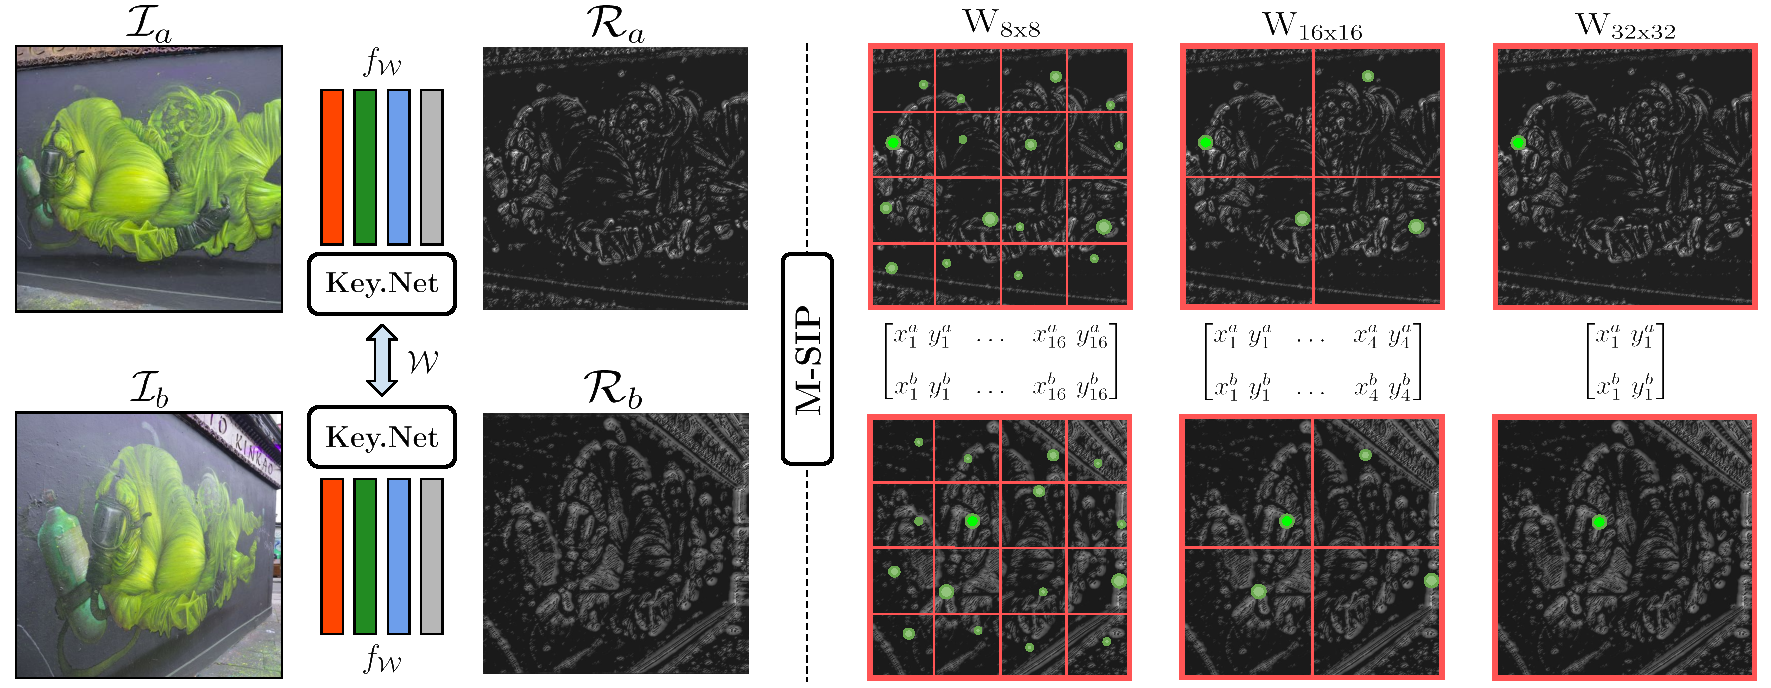
\includegraphics[width=\linewidth]{main/chapter02/figures/training_v2.pdf}
    \vspace{-0.20cm}
    \caption[Siamese training process]{\textbf{Siamese training process.} Image $I_a$ and $I_b$ go through Key.Net to generate their response maps, $R_a$ and $R_b$. M-SIP proposes interest point coordinates for each one of the windows at multi-scale regions. The final loss function is computed as a regression of coordinate indexes from $I_a$ and transformed coordinate indexes from $I_b$ (see in equation~\ref{eq:context_losses}).}
    \label{keynet_fig:trainingfigure}
\end{figure}

\begin{figure}
\vspace{-0.10cm}
 \hspace*{-0.4cm} 
 \centering
   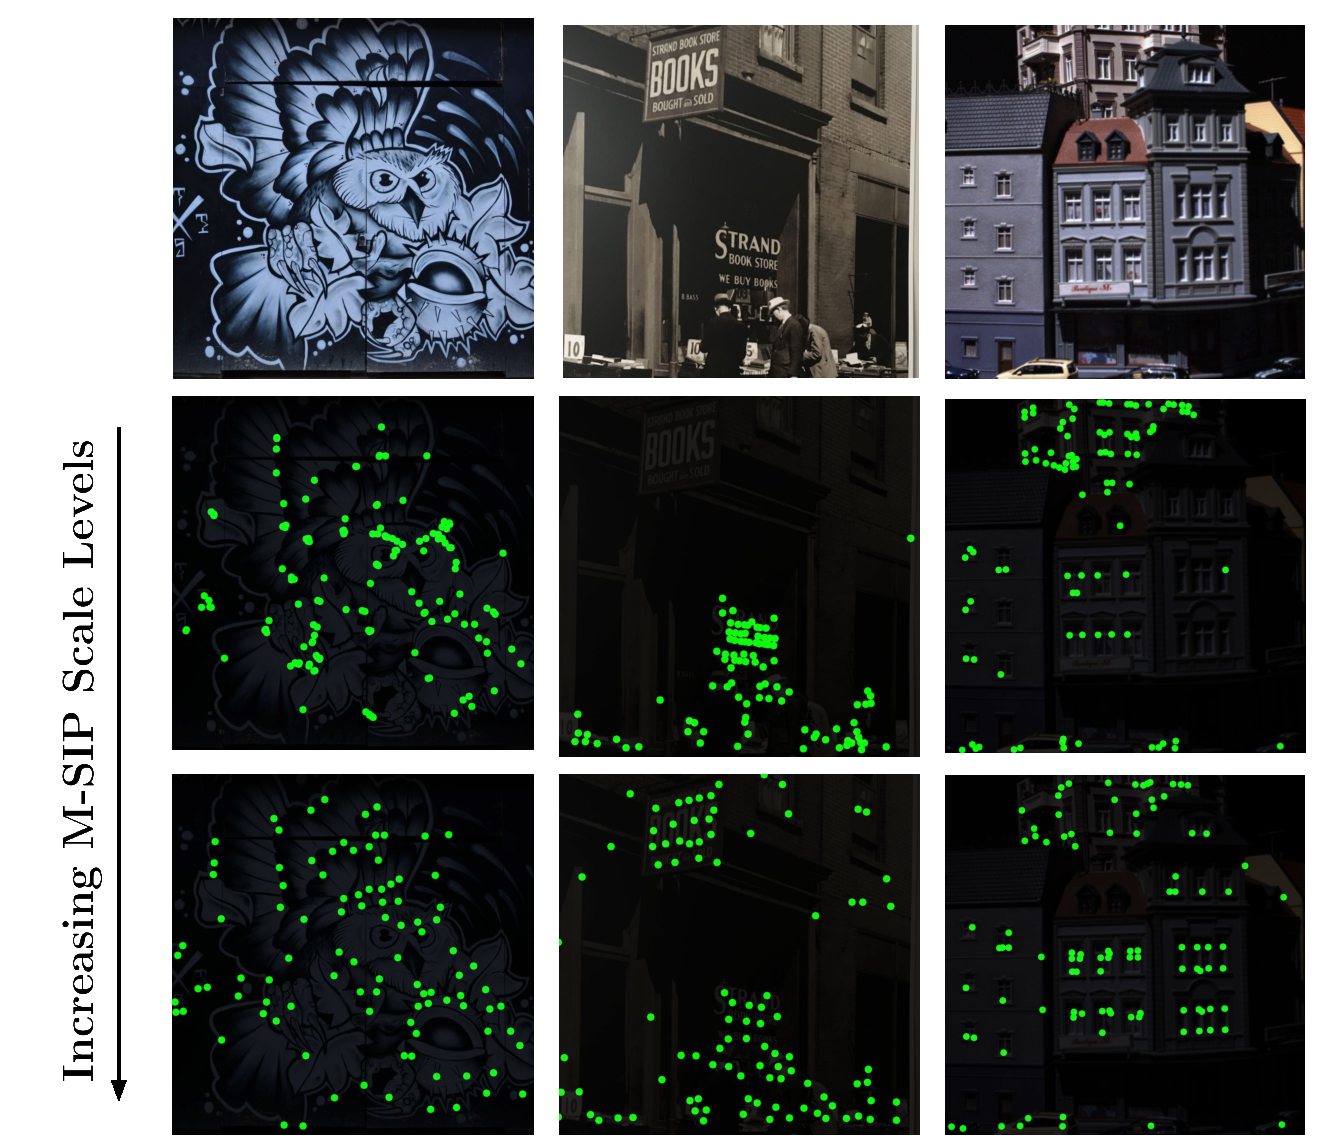
\includegraphics[width=\linewidth]{main/chapter02/figures/M-SIP_Scale_Levels_v5.pdf}
   \vspace{-0.2cm}
    \caption[Key.Net qualitative results with different windows sizes]{\textbf{Key.Net qualitative results with different windows sizes.} Keypoints obtained after adding larger context windows to M-SIP operator. The points that are more stable remain as the M-SIP operator increases its window size. While the feature maps in the middle row contain points around edges or non discriminative areas from the initial scales, the bottom row shows detections from the lower scales which shows that are more robust under geometric transformations.}
    \label{fig:M-SIP_Scale_Levels}
\end{figure}

\subsubsection{Multi-scale Index Proposal Layer}
\label{keynet_sec:multi_index_proposal_layer}

IP layer returns one location per window, therefore, the number of keypoints per image strongly depends on the predefined window size $N$. In particular, if N is big with an increasing size only a few dominant keypoints survive in the image. In \cite{DSPSIFT_soatto}, authors demonstrated improved performance of local features by accumulating image features not only within a spatial window but also within the neighboring scales. We propose to extend IP layer loss by incorporating multi-scale representation of a local neighborhood. Multiple window sizes encourage the network to find keypoints that exist across a range of scales. The additional benefit of including larger windows is that other keypoints within the window can act as anchors for the estimated location of the dominant keypoint. Similar idea proved successful in~\cite{Local_affine_frames_Matas}, where stable region boundaries are used.

We, therefore, propose the Multi-Scale Index Proposal (M-SIP) layer. M-SIP splits multiple times the response map into grids, each with a window size of $N_s \times N_s$ and computes the candidate keypoint position for each window as shown in figure~\ref{keynet_fig:trainingfigure}. Our proposed loss function is the average of covariant constraint losses from all scale levels: 
\begin{equation}
\mathbf{L}_{MSIP}(I_{a}, I_{b}, H_{a,b}) =  \sum_{\substack{s}}\lambda_{s} \mathbf{L}_{IP}(I_{a}, I_{b}, H_{a,b},N_s),
  \label{eq:context_losses_m}
\end{equation}
where $s$ is the index of the scale level with $N_s$ as window size, $\mathbf{L}_{IP}$ is the covariant constraint loss and $\lambda_{s}$ is the control parameter at scale level $s$, that decreases proportionally to the increasing window area as larger windows lead to a larger loss, which is somewhat similar to the scale-space normalisation~\cite{mikolajczykIJCV2004}. \par 

The combination of different scales imposes an intrinsic process of simultaneous scoring and ranking of keypoints within the network. In order to minimize the loss, the network will learn to give higher scores to the pixel locations centered on image features that remain dominant across a range of scales. Figure~\ref{fig:M-SIP_Scale_Levels} shows different response maps for increasing window size.

\begin{figure}
 \hspace*{-0.1cm} 
 \vspace{-0.4cm}
    \centering
    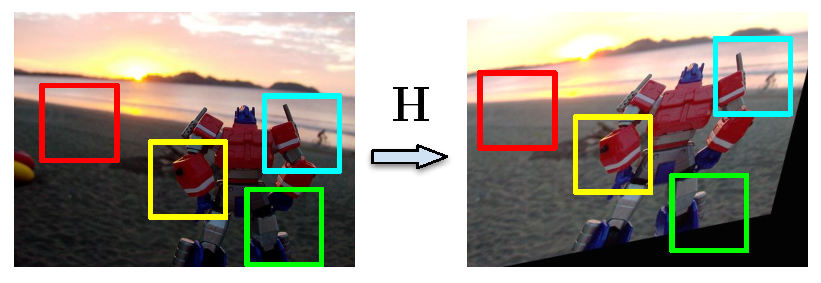
\includegraphics[width=\linewidth]{main/chapter02/figures/dataset_v3.pdf}
    \vspace{-0.0cm}
    \caption[Homography synthetic data generation]{\textbf{Homography synthetic data generation.} We apply random geometric and photometric transformations to images and extract pairs of corresponding regions as the training set. Red crop is discarded by checking the response of the handcrafted filters.}
    \label{fig:dataset}
\end{figure}

\subsection{Experimental Evaluation}
\label{keynet_sec:experimental_evaluation}

%----------------------------------------------------------------------------------------
%	Section: Experimental Evaluation
%----------------------------------------------------------------------------------------

In this section, we present implementation details, metrics and the dataset used for evaluating the method.
%----------------------------------------------------------------------------------------
%	Subsubsection: Creating the Training Dataset
%----------------------------------------------------------------------------------------

\subsubsection{Training Data}
\label{sec:create_dataset}

We generate a synthetic training set from ImageNet ILSVRC 2012 \cite{RussakovskyDSKSMHKKBBF14} dataset. We apply random geometric transformations to images and extract pairs of corresponding regions as our training set. The process is illustrated in figure~\ref{fig:dataset}. The parameters of the transformations are: scale $[0.5, 3.5]$, skew  $[-0.8, 0.8]$ and rotation $[-60\degree, 60\degree]$ which are common transformations seen across scene reconstruction datasets. Textureless regions are discarded by checking if the mean response of any of the handcrafted filters is lower than a threshold. We modify contrast, brightness and hue value in HSV space to one of the images to improve network's robustness against illumination changes. In addition, for each pair, we generate a binary mask that indicates the common area between images. Mask is used in training to avoid regressing indexes of keypoints that are not present in the common region. There are 12,000 image pairs of size 192 $\times$ 192. We use 9,000 of them as the training data and 3,000 as validation set.

%----------------------------------------------------------------------------------------
%	Subsection: Evaluation Metric and Dataset
%----------------------------------------------------------------------------------------

\subsubsection{Evaluation Metrics}
\label{subsec:Evaluation}

We follow the evaluation protocol proposed in \cite{mikolajczykpami2005} and improved in the follow up works~\cite{LIFT,Karel_Vedaldi_ECCV_16,Zhang_Felix_CVPR_17,Karel_Vedaldi_BMVC_18} which is based on the repeatability scores. The repeatability score for a pair of images is computed as the ratio between the number of corresponding keypoints and the lower number of keypoints detected in one of the two images. We take the top-k extracted keypoints to compare across methods and allow each keypoint to match only once as in \cite{FASTER, TILDE}. In addition, as exposed by \cite{Karel_Vedaldi_BMVC_18}, we address the bias from the magnification factor that was applied to accelerate the computation of the overlap error between multi-scale keypoints.

Keypoints are identified by spatial coordinates and scales at which the features were detected, the last defined by a squared around the center.  To identify corresponding keypoints we compute the Intersection-over-Union error, $\epsilon_{IoU}$, between the areas of the two candidates. To evaluate the accuracy of keypoint location and scale independently, we perform two sets of experiments. One is based on the scales extracted from the scale space and the other assumes the scales are correctly detected by using the ground truth parameters. In our benchmark, we use top 1,000 interest points that belong to the common region between images and a match is considered correct when $\epsilon_{IoU}$ is smaller than 0.4 i.e., the overlap between corresponding regions is more than 60\%. The scales are normalized as in \cite{Karel_Vedaldi_BMVC_18}, which sets the larger size in a pair of points to 30 pixels, and rescales the other one accordingly. Non-maxima suppression of $15 \times 15$ is performed at inference time during evaluation.

HPatches~\cite{HPatches} dataset is used for testing. HPatches contains 116 sequences, which are split between viewpoint and illumination transformations, 59 and 57 sequences respectively. HPatches offers predefined image patches for evaluating descriptors, instead, we use full images for evaluating keypoint detectors. 

%----------------------------------------------------------------------------------------
%	Subsection: Implementation Details
%----------------------------------------------------------------------------------------

\subsubsection{Experimental Setup}
\label{subsec:Implementation_Details}
Training is performed in a siamese pipeline, with two instances of Key.Net that share the weights and are updated at the same time. Each convolutional layer has $M$ = 8 filters of size $5 \times 5$, with He~\cite{HE_initializatio} weights initialization and L2 kernel regularizer. We compute the covariant constraint loss $\mathbf{L}_{M\mbox{-}SIP}$ for five scale levels, with the size of the M-SIP windows $N_s \in [8, 16, 24, 32, 40]$ and loss term $\lambda_s \in [256, 64, 16, 4, 1]$, that were determined by performing a hyperparameter search on the validation set. Larger candidate window sizes have greater mean errors between coordinate points since the maximum distance is proportional to the window size. Thus, $\lambda_s$ has the largest value for the smallest window. We use a batch size of 32, an Adam Optimizer with a learning rate of $10^{-3}$ and a decay factor of 0.5 after 30 epochs. On average, the architecture converges in 20 epochs, 2h on a machine with an i7-7700 CPU running at 3.60GHz and a NVIDIA GeForce GTX 1080 Ti. Evaluation benchmark, synthetic data generator, Key.Net network, and loss are implemented using TensorFlow and are available on GitHub\footnote{https://github.com/axelBarroso/Key.Net}. 


\begin{figure}
\vspace{-0.10cm}
    \centering
    % https://repl.it/@edgarriba/repeatabilitykeypointnet
    % \vspace{-3.0cm}
    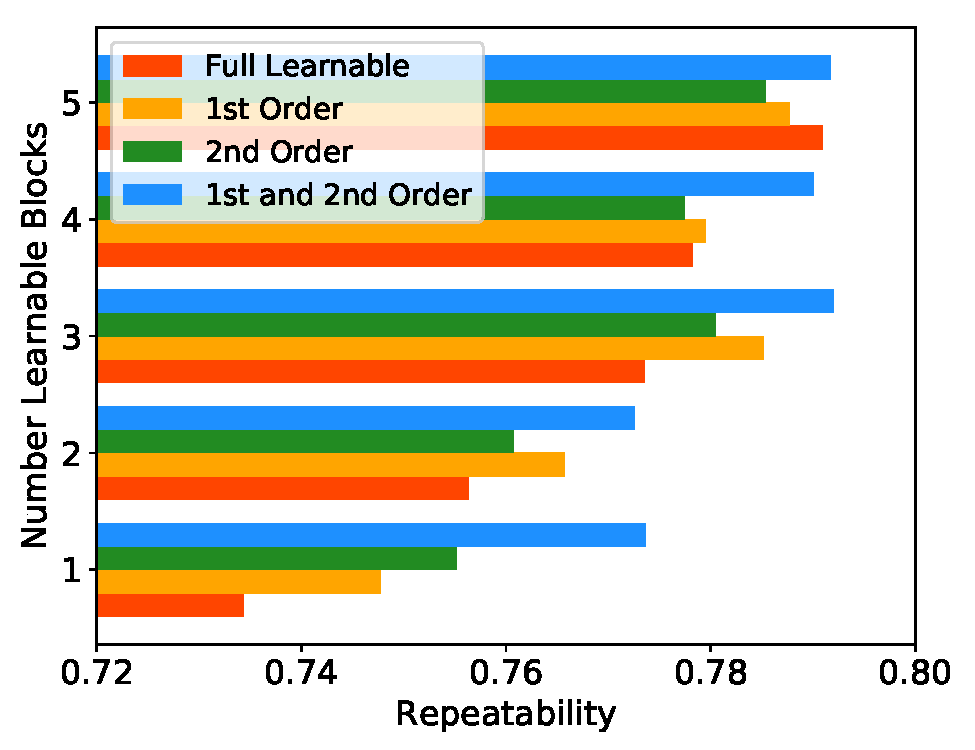
\includegraphics[width=0.65\linewidth]{main/chapter02/figures/learnable_blocks.pdf}
\caption[Key.Net quantitative results for different learnable blocks]{\textbf{Key.Net quantitative results for different learnable blocks.} Repeatability results for different combinations of handcrafted filters and a number of learnable layers ($M=8$ filters each). A higher number of layers leads to better results. All repeatability scores are computed on synthetic validation set from ImageNet.}
\label{fig:keynet_learnableblocks}
\end{figure}


\begin{table}
\vspace{-0.10cm}
    \centering
    \begin{tabular}{ccccclc}
        \hline
        \multicolumn{5}{c}{M-SIP Region Sizes} & \multicolumn{1}{c}{} & \multicolumn{1}{c}{}\\ 
        \cline{1-5} 
        W{$_{8\text{x}8}$} & W{$_{16\text{x}16}$} & W$_{24\text{x}24}$ & W$_{32\text{x}32}$ & W$_{40\text{x}40}$ & & Repeatability \\
        \hline
        \checkmark & - & - & - & - && 70.5  \\
        \checkmark & \checkmark & - & - & - && 74.6  \\
        \checkmark & \checkmark & \checkmark & - & - && 76.8  \\
        \checkmark & \checkmark & \checkmark & \checkmark & - && 77.6  \\
        - & - & - & - & \checkmark && 65.7 \\
        - & - & - & \checkmark & \checkmark && 71.4 \\
        - & - & \checkmark & \checkmark & \checkmark && 73.2  \\
        - & \checkmark & \checkmark & \checkmark & \checkmark && 74.9  \\
        \checkmark & \checkmark & \checkmark & \checkmark & \checkmark && \textbf{79.1}  \\
        % \hline
    \end{tabular}
\caption[Key.Net quantitative results for M-SIP regions sizes]{\textbf{Key.Net quantitative results for M-SIP regions sizes.} Comparison of repeatability results for the various number of levels in M-SIP operator. We show different combinations of context losses as the final loss,  from smaller to larger regions. The best result is obtained when using five window sizes from $8\times 8$ up to $40\times 40$.}
\label{table:keynet_region_sizes}
\end{table}

\subsection{Detection Results}
\label{keynet_sec:results}

%----------------------------------------------------------------------------------------
%	Section: Experiments
%----------------------------------------------------------------------------------------
In this section, we present the experiments and discuss the results. We first show results on validation data for several variants of the proposed architecture. Next, Key.Net repeatability scores in single-scale and multi-scale are presented along with the state-of-the-art detectors on HPatches. Moreover, we evaluate the matching performance, the number of learnable parameters and inference time of our proposed detector and compare to other techniques.

\subsubsection{Preliminary Analysis}

\label{subsec:preliminary_analysis}
We study several combinations of loss terms, different handcrafted filters and the effects of the number of learnable layers or pyramid levels within the architecture.

\begin{itemize}
    \item \textbf{Filter Combinations} are analyzed in figure~\ref{fig:keynet_learnableblocks}. We show results for $1^{st}$ and $2^{nd}$ order filters as well as their combination. All networks have the same number of filters, however, we either freeze first layer of 10 filters with handcrafted kernels (c.f. section \ref{sec:handcrafted_filters}) or learn them depending on the variant of our network, e.g, in Fully Learnable Key.Net there are no handcrafted filters as all are randomly initialized and learned. The results show that the information provided by handcrafted filters is essential when the number of learnable layers is small. Handcrafted filters act as soft constraints, which directly discard areas without gradients, i.e. non-discriminative with low repeatability. However, as we add more learnable blocks, repeatability scores for combined and fully learnable networks become comparable. Naturally, gradient-based handcrafted filters are simple, and architectures with enough complexity can learn them. %However, the use of engineered features leads to a smaller architecture while maintaining the performance, which is often critical for real-time applications. In summary, combining both types of filters allows to significantly reduce the number of learnable layers. We use Key.Net architecture with three learnable blocks in the following experiments.
    \item \textbf{Multiple Pyramid Levels} at the input to the network also affect the detection performance as shown in table~\ref{table:keynet_region_sizes}. For a single pyramid level, only the original image is used as input. Adding pyramid levels is similar to increasing the size of the receptive fields in the architecture. Our experiment suggests that using more than three levels does not lead to significantly improved results. On the validation set, we obtain a repeatability score of 72.5\% for one level,  an increase of 6.6\% for three, and 7.0\% for five levels. We, therefore, use three levels, which achieve good performance while keeping the computational cost low.
\end{itemize}

\subsubsection{Detection algorithm comparison}

This section presents the results for state-of-the-art local feature detectors along with our proposed method. Table \ref{table:repeatability_scores} shows the repeatability score,  average intersection-over-union error $\Bar{\epsilon}_{IoU}$.  Suffixes -TI and -SI, refer to translation (detection at a single scale only) and scale invariance (detection at multiple scales), respectively. Keypoint location is only evaluated under L by assuming correct scale detection, while scale and location (SL) use the actual detected scale and location for computing the overlap error.

In addition to Key.Net, we evaluate in these experiment the performance of Tiny-Key.Net, which is a reduced size architecture with all handcrafted filters but only one learnable layer with one filter  ($M = 1$) and a single downscaling factor in the input. The idea behind Tiny-Key.Net is to demonstrate how far the complexity can be reduced while keeping good performance. Key.Net and Tiny-Key.Net are extended to scale invariance by evaluating the detector on several scaled images, similar to \cite{Zhang_Felix_CVPR_17}. We also show results on single scale input Key.Net-TI, to compare it directly with other TI detectors such as SuperPoint or TILDE. We manually set the threshold of algorithms to return at least 1,000 points per image. As MSER proposes regions without scoring or ranking, we randomly pick 1,000 points to compute the results. We repeat this experiment ten times and average the results for MSER. Key.Net has the best results on viewpoint sequences, in terms of both, location and scale. Tiny-Key.Net does not perform as well as Key.Net but it is within the top three repeatability scores, after Key.Net-TI and Key.Net-SI.

% \begin{landscape}
% \begin{figure}[!tbh]
%  \hspace*{-0.1cm} 
%  \vspace{-0.4cm}
%     \centering
%     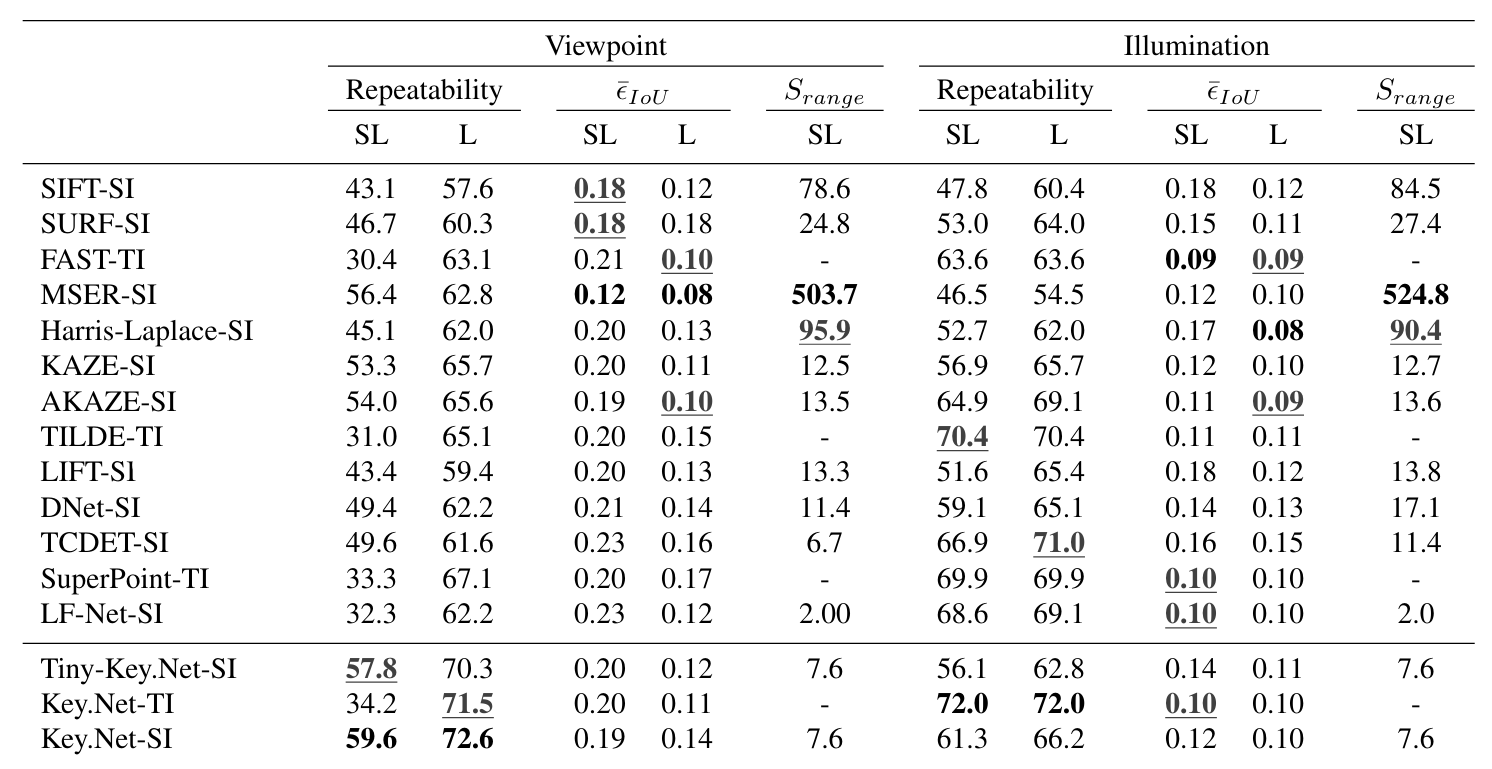
\includegraphics[scale=0.3]{main/chapter02/figures/keynet_repeatability_results.png}
%     \vspace{-0.0cm}
%     \caption[Key.Net repeteability results]{\textbf{Key.Net repeteability results.} Repeatability results (\%) for translation (TI) and scale (SI) invariant detectors on HPatches. We also report average overlap error $\Bar{\epsilon}_{IoU}$ and ratio of maximum to minimum extracted scale $S_{Range}$. In SL, scales and locations are used to compute overlap error, meanwhile, in L, only locations are used and scales are assumed to be correctly estimated. Key.Net and Tiny-Key.Net are the best algorithms on viewpoint, for both L and SL. On illumination sequences, translation invariant Key.Net-TI obtains the best accuracy. Among scale invariant SI detectors, TCDNET is the best in L and LF-Net in SL.}
%     \label{fig:repeatability_scores}
% \end{figure}
% \end{landscape}

On illumination sequences, Key.Net-TI performs the best among TI detectors, which are not affected by scale estimation errors. TCDET, which uses points detected by TILDE as anchors, is the most accurate in location estimation compared to other SI detectors. Note that TILDE based detectors were specifically designed and trained for illumination sequences. LF-Net is the best SI detector according to SL overlap, not suffering much from incorrect scale estimations. %However, its repeatability decreases the most from L to SL among all SI detectors on viewpoint sequences. Key.Net-SI addresses the scale changes better than the other methods but the errors in multi-scale sampling affect it when there is no scale change between images i.e. illumination sequences. This has often been observed for detectors with more invariance than required by the data. Handcrafted detectors have the lowest average overlap error $\Bar{\epsilon}_{IoU}$ among all detectors.
%A wide range of scales $S_{range}$ is detected by MSER, which has a great capability of extracting local features from different scales due to its feature segmentation nature.

\begin{landscape}
\begin{table}
\vspace{-0.10cm}
\begin{center}
\begin{tabular}{lccccccclccccccc}
\hline
\noalign{\smallskip}
\multicolumn{1}{c}{} & \multicolumn{7}{c}{Viewpoint} & \multicolumn{1}{c}{} & \multicolumn{7}{c}{Illumination} \\ 
\cline{2-8} \cline{10-16} \noalign{\smallskip}
\multicolumn{1}{c}{} & \multicolumn{2}{c}{Repeatability} && \multicolumn{2}{c}{$\Bar{\epsilon}_{IoU}$} && \multicolumn{1}{c}{$S_{range}$} & \multicolumn{1}{c}{} & \multicolumn{2}{c}{Repeatability} && \multicolumn{2}{c}{$\Bar{\epsilon}_{IoU}$} && \multicolumn{1}{c}{$S_{range}$} \\
\cline{2-3} \cline{5-6} \cline{8-8} \cline{10-11}  \cline{13-14} \cline{16-16} \noalign{\smallskip}
 & SL & L && SL & L && SL && SL & L && SL & L && SL \\
\noalign{\smallskip}
\hline
\noalign{\smallskip}
SIFT-SI \cite{SIFT}                    & 43.1 & 57.6 && \textbf{\textcolor{darkgray}{\underline{0.18}}} & 0.12 && 78.6 && 47.8 & 60.4 && 0.18 & 0.12 && 84.5 \\
SURF-SI \cite{SURF}                    & 46.7 & 60.3 && \textbf{\textcolor{darkgray}{\underline{0.18}}} & 0.18 && 24.8 && 53.0 & 64.0 && 0.15 & 0.11 && 27.4 \\
FAST-TI \cite{FAST}                    & 30.4 & 63.1 && 0.21 & \textbf{\textcolor{darkgray}{\underline{0.10}}} && - && 63.6 & 63.6 && \textbf{0.09} & \textbf{\textcolor{darkgray}{\underline{0.09}}} && - \\
MSER-SI \cite{MSER}                    & 56.4 & 62.8 && \textbf{0.12} & \textbf{0.08} && \textbf{503.7} && 46.5 & 54.5 && 0.12 & 0.10 && \textbf{524.8} \\
Harris-Laplace-SI \cite{HarrisLaplace} & 45.1 & 62.0 && 0.20 & 0.13 && \textbf{\textcolor{darkgray}{\underline{95.9}}} && 52.7 & 62.0 && 0.17 & \textbf{0.08} && \textbf{\textcolor{darkgray}{\underline{90.4}}} \\
KAZE-SI \cite{KAZE}                    & 53.3 & 65.7 && 0.20 & 0.11 && 12.5 && 56.9 & 65.7 && 0.12 & 0.10 && 12.7 \\
AKAZE-SI \cite{AKAZE}                  & 54.0 & 65.6 && 0.19 & \textbf{\textcolor{darkgray}{\underline{0.10}}} && 13.5 && 64.9 & 69.1 && 0.11 & \textbf{\textcolor{darkgray}{\underline{0.09}}} && 13.6 \\
TILDE-TI \cite{TILDE}                  & 31.0 & 65.1 && 0.20 & 0.15 && - && \textbf{\textcolor{darkgray}{\underline{70.4}}} & 70.4 && 0.11 & 0.11 && - \\
LIFT-SI \cite{LIFT}                    & 43.4 & 59.4 && 0.20 & 0.13 && 13.3 && 51.6 & 65.4 && 0.18 & 0.12 && 13.8 \\
DNet-SI \cite{Karel_Vedaldi_ECCV_16}   & 49.4 & 62.2 && 0.21 & 0.14 && 11.4 && 59.1 & 65.1 && 0.14 & 0.13 && 17.1 \\
TCDET-SI \cite{Zhang_Felix_CVPR_17}    & 49.6 & 61.6 && 0.23 & 0.16 && 6.7 && 66.9 & \textbf{\textcolor{darkgray}{\underline{71.0}}} && 0.16 & 0.15 && 11.4 \\
SuperPoint-TI \cite{detone2017superpoint} & 33.3 & 67.1 && 0.20 & 0.17 && - && 69.9 & 69.9 && \textbf{\textcolor{darkgray}{\underline{0.10}}} & 0.10 && - \\
LF-Net-SI \cite{OnoSerra18}            & 32.3 & 62.2 && 0.23 & 0.12 && 2.00 && 68.6 & 69.1 && \textbf{\textcolor{darkgray}{\underline{0.10}}} & 0.10 && 2.0 \\
\noalign{\smallskip}
\hline
\noalign{\smallskip}
Tiny-Key.Net-SI & \textbf{\textcolor{darkgray}{\underline{57.8}}} & 70.3 && 0.20 & 0.12 && 7.6 && 56.1 & 62.8 && 0.14 & 0.11 && 7.6 \\
Key.Net-TI & 34.2 & \textbf{\textcolor{darkgray}{\underline{71.5}}} && 0.20 & 0.11 && - && \textbf{72.0} & \textbf{72.0} && \textbf{\textcolor{darkgray}{\underline{0.10}}} & 0.10 && - \\

Key.Net-SI & \textbf{59.6} & \textbf{72.6} && 0.19 & 0.14 && 7.6 && 61.3 & 66.2 && 0.12 & 0.10 && 7.6 \\
\end{tabular}
%\vspace{-0.2cm}
\caption[Key.Net repeteability results]{\textbf{Key.Net repeteability results.} Repeatability results (\%) for translation (TI) and scale (SI) invariant detectors on HPatches. We also report average overlap error $\Bar{\epsilon}_{IoU}$ and ratio of maximum to minimum extracted scale $S_{Range}$. In SL, scales and locations are used to compute overlap error, meanwhile, in L, only locations are used and scales are assumed to be correctly estimated. Key.Net and Tiny-Key.Net are the best algorithms on viewpoint, for both L and SL. On illumination sequences, translation invariant Key.Net-TI obtains the best accuracy.}
\label{table:repeatability_scores}
\end{center}
\end{table}
\end{landscape}

\begin{table}[!tbh]
\vspace{-0.10cm}
\begin{center}
\begin{tabular}{lcc}
\hline
\noalign{\smallskip}
% \multicolumn{3}{c}{\textbf{Descriptor Matching Score}} \\ 
% \hline
\multicolumn{1}{c}{} & \multicolumn{2}{c}{Matching Score} \\ 
\cline{2-3} \noalign{\smallskip}
\multicolumn{1}{c}{} & \multicolumn{1}{c}{View} & \multicolumn{1}{c}{Illum} \\
\noalign{\smallskip}
\hline
\noalign{\smallskip}
MSER \cite{MSER} + HardNet \cite{Mishchuk_Mishkin_NIPS17}   & 11.7 & 18.8 \\
SIFT \cite{SIFT} + HardNet \cite{Mishchuk_Mishkin_NIPS17}   & 23.2 & 24.8 \\
% FAST \cite{SIFT} + HardNet \cite{Mishchuk_Mishkin_NIPS17}   & 19.7 & 40.5 \\
HarrisLaplace \cite{HarrisLaplace} + HardNet \cite{Mishchuk_Mishkin_NIPS17} & 30.0 & 31.7 \\
% KAZE \cite{KAZE} + HardNet \cite{Mishchuk_Mishkin_NIPS17} & 32.2 & 39.4 \\
AKAZE \cite{AKAZE} + HardNet \cite{Mishchuk_Mishkin_NIPS17} & 36.4 & 41.4 \\
TILDE \cite{TILDE} + HardNet \cite{Mishchuk_Mishkin_NIPS17} & 32.3 & 40.3 \\
LIFT \cite{LIFT} + HardNet \cite{Mishchuk_Mishkin_NIPS17} & 30.3 & 32.8 \\
DNet \cite{Karel_Vedaldi_ECCV_16} + HardNet \cite{Mishchuk_Mishkin_NIPS17} & 33.5 & 34.7 \\
TCDET \cite{Zhang_Felix_CVPR_17} + HardNet \cite{Mishchuk_Mishkin_NIPS17} & 27.6 & 36.3 \\
SuperPoint \cite{detone2017superpoint} + HardNet \cite{Mishchuk_Mishkin_NIPS17} & 37.4 & \textbf{\textcolor{darkgray}{\underline{43.0}}} \\
LF-Net \cite{OnoSerra18} + HardNet \cite{Mishchuk_Mishkin_NIPS17} & 26.9 & \textbf{43.8} \\
\noalign{\smallskip}
\hline
\noalign{\smallskip}
LIFT \cite{LIFT} & 21.8 & 26.5 \\
SuperPoint \cite{detone2017superpoint} & \textbf{\textcolor{darkgray}{\underline{38.0}}} & 41.5 \\
LF-Net \cite{OnoSerra18} & 23.0 & 29.1 \\
\noalign{\smallskip}
\hline
\noalign{\smallskip}
Tiny-Key.Net + HardNet \cite{Mishchuk_Mishkin_NIPS17} & 37.9 & 37.3 \\
Key.Net + HardNet \cite{Mishchuk_Mishkin_NIPS17}      & \textbf{38.4} & 40.7 \\
\end{tabular}
\caption[Key.Net matching scores results]{\textbf{Key.Net matching scores results.} Matching score (\%) of best detectors together with HardNet and state-of-the-art detector/descriptors. Results on HPatches sequences, both viewpoint, and illumination. Key.Net architecture get the best matching score for viewpoint, while LF-Net+HardNet for illumination sequences.}
\label{table:matchingScore}
\end{center}
\end{table}


\subsubsection{Keypoint matching analysis}
In order to demonstrate that the detected features are useful for matching, table \ref{table:matchingScore} shows the percentage of keypoints that have been put in correspondence matching scores for the different detectors combined with HardNet  descriptor \cite{Mishchuk_Mishkin_NIPS17}. As our method only focuses on the detection part, and for a fair comparison, we used the same descriptor and discard the orientation for all methods that provide it since our method do not estimate the keypoint orientation. In addition, we include in the table  LIFT\cite{LIFT}, SuperPoint\cite{detone2017superpoint} and LF-Net\cite{OnoSerra18} with their descriptors, but ignoring their orientation estimation. The matching score is computed as the ratio between features matched and detected top 1k best ranked points. Best matching percentages matching scores are obtained by Key.Net on viewpoint, and LF-Net+HardNet on illumination. Feature detectors that were optimized jointly with a descriptor \cite{LIFT, detone2017superpoint, OnoSerra18} have better matching score than regular learned detectors on illumination sequences, but not on viewpoint. Handcrafted AKAZE performs close to the top learned methods.\par


\subsubsection{Efficiency}
We also compare the number of learnable parameters, indicating then the complexity of the predictor, therefore, an increased risk of overfitting and a need for large training data. Table~\ref{table:number_parameters} shows the approximate number of parameters for different architectures. 
Learnable parameters that are not used during inference in the detector part are not counted for SuperPoint and LF-Net detectors.
The highest complexity is from SuperPoint with $940k$ learnable parameters. Key.Net has nearly 160 times fewer parameters and Tiny-Key.Net has $3$,$100$ times fewer parameters than SuperPoint with better repeatability for viewpoint scenes.
%the running time of our two proposed architectures, Tiny-Key.Net and Key.Net.
% We proposed Tiny-Key.Net to demonstrate how far the network's complexity can be reduced while still keeping good performance. 
The inference time of an image of 600 $\times$ 600 is 5.7ms (175 FPS) and 31ms (32.25 FPS) for Tiny-Key.Net and Key.Net, respectively. 


\begin{table}[!tbh]
\vspace{-0.10cm}
\begin{center}
\begin{tabular}{ccccc}
\hline
\noalign{\smallskip}
\multicolumn{5}{c}{Number of Learnable Parameters} \\ 
\cline{1-5} \noalign{\smallskip}
\scalebox{0.92}{TCDET} & \scalebox{0.92}{SuperPoint} & \scalebox{0.92}{LF-Net} & \scalebox{0.92}{Key.Net} & \scalebox{0.92}{Tiny-Key.Net}\\
\hline
\noalign{\smallskip}
548k & 940k & 39k & \textbf{\textcolor{darkgray}{\underline{5.9k}}} & \textbf{280} \\
\noalign{\smallskip}
% \hline
\noalign{\smallskip}
\vspace{-0.75cm}
\end{tabular}
\caption[Key.Net number of parameters comparison]{\textbf{Key.Net number of parameters comparison.} Comparison of the number of learnable parameters for state-of-the-art architectures. Tiny-Key.Net has only one learnable block with one filter.}
\label{table:number_parameters}
\end{center}
\end{table}


\subsection{Conclusions}
In this section we introduced an approach to detect local features that combines handcrafted and learned CNN filters that can be easily replaced by any existing detection method in the reconstruction pipeline. We have proposed a multi-scale index proposal layer that finds keypoints across a range of scales, with a loss function that optimizes the robustness and discriminating properties of the detections. We demonstrated how to compute and combine differentiable keypoint detection loss for multi-scale representation. Evaluation results on large benchmark show that combining handcrafted and learned features as well as multi-scale analysis at different stages of the network improves the repeatability scores compared to other state-of-the-art keypoint detection methods. We further show that using handcrafted filters significantly reduce the complexity of the architecture leading to a detector with 280 learnable parameters and inference of 175 frames per second.